\documentclass[11pt,a4paper]{article}

% --- Paquetes ---
\usepackage[T1]{fontenc}
\usepackage[utf8]{inputenc}
\usepackage[spanish,es-tabla]{babel}
\usepackage[margin=2.5cm]{geometry}
\usepackage{graphicx}
\usepackage{xcolor}
\usepackage{tcolorbox}
\tcbuselibrary{skins}
\usepackage{hyperref}
\usepackage{fancyhdr}
\usepackage{float}
\usepackage{booktabs}
\usepackage{titlesec}
\usepackage{enumitem}

% --- Colores institucionales y estilo de código ---
\definecolor{unsaacblue}{RGB}{18, 52, 102}
\definecolor{terminalbg}{RGB}{24, 24, 27}
\definecolor{terminalborder}{RGB}{63, 63, 70}
\definecolor{codebg}{RGB}{248, 249, 250}

\hypersetup{
    colorlinks=true,
    linkcolor=unsaacblue,
    filecolor=unsaacblue,
    urlcolor=unsaacblue,
    citecolor=unsaacblue
}

% --- Encabezados y Pies de página ---
\pagestyle{fancy}
\fancyhf{}
\fancyhead[L]{\small\textbf{UNSAAC} - Ingeniería de Software}
\fancyhead[R]{\small\textbf{Laboratorio 1}: Entorno de Desarrollo y Git}
\fancyfoot[L]{\small Edmil Jampier Saire Bustamante}
\fancyfoot[R]{\thepage}
\renewcommand{\headrulewidth}{0.8pt}
\renewcommand{\footrulewidth}{0.4pt}

% --- Formato de títulos ---
\titleformat{\section}{\Large\bfseries\color{unsaacblue}}{\thesection.}{0.5em}{}[\titlerule]
\titleformat{\subsection}{\large\bfseries\color{unsaacblue}}{\thesubsection.}{0.5em}{}

% --- Bloque de comandos (Estilo terminal) ---
\newtcolorbox{terminalbox}[1]{
    colback=terminalbg,
    colframe=terminalborder,
    coltext=white,
    fontupper=\small\ttfamily,
    title={\small\textbf{#1}},
    arc=3mm,
    boxrule=1pt,
    left=8pt, right=8pt, top=8pt, bottom=8pt,
    enhanced,
    attach boxed title to top left={xshift=5mm, yshift=-3mm},
    boxed title style={colback=unsaacblue, colframe=unsaacblue, arc=2mm}
}

\begin{document}

% ==============================================================================
% CARÁTULA
% ==============================================================================
\begin{titlepage}
    \centering
    {\Large\textbf{UNIVERSIDAD NACIONAL DE SAN ANTONIO ABAD DEL CUSCO}}\\[0.3cm]
    {\large\textbf{FACULTAD DE INGENIERÍA ELÉCTRICA, ELECTRÓNICA, INFORMÁTICA Y MECÁNICA}}\\[0.2cm]
    {\large\textbf{ESCUELA PROFESIONAL DE INGENIERÍA INFORMÁTICA Y DE SISTEMAS}}\\[1.2cm]

    
\includegraphics[height=4.2cm,keepaspectratio]{capturas/logo_unsaac.png}\\[1.2cm]

    {\LARGE\bfseries\color{unsaacblue} INFORME DE LABORATORIO N$^\circ$ 1}\\[0.4cm]
    {\Large\textbf{Introducción al Entorno de Desarrollo y Control de Versiones con Git}}\\[1.4cm]

    \begin{minipage}{0.85\textwidth}
        \large
        \textbf{Asignatura:} Ingeniería de Software \\[0.25cm]
        \textbf{Docente:} Ing. Lisha Sabah Diaz Caceres \\[0.25cm]
        \textbf{Alumno:} Edmil Jampier Saire Bustamante \\[0.25cm]
        \textbf{Código:} 174449 \\[0.25cm]
        \textbf{Correo:} \href{mailto:174449@unsaac.edu.pe}{174449@unsaac.edu.pe} \\[0.25cm]
        \textbf{Repositorio en GitHub:} \href{https://github.com/milith0kun/pedidos-comida-cusco}{github.com/milith0kun/pedidos-comida-cusco}
    \end{minipage}

    \vfill
    {\large\textbf{Cusco -- Perú}}\\[0.2cm]
    {\large 2026}
\end{titlepage}

\newpage
\tableofcontents
\newpage

% ==============================================================================
% 1. OBJETIVO
% ==============================================================================
\section{Objetivo}
Configurar mi entorno de desarrollo local con Git, practicar los comandos fundamentales de control de versiones en un proyecto nuevo y sincronizarlo con un repositorio remoto en GitHub.

% ==============================================================================
% 2. RESULTADOS DE APRENDIZAJE
% ==============================================================================
\section{Resultados de Aprendizaje}
\begin{itemize}[leftmargin=1.5cm]
    \item Comprender por qué el control de versiones es indispensable para desarrollar software de manera ordenada.
    \item Configurar las credenciales de usuario en Git desde la terminal.
    \item Gestionar el ciclo de vida de un proyecto con comandos locales (\texttt{git init}, \texttt{git add}, \texttt{git commit}) y remotos (\texttt{git remote}, \texttt{git push}).
\end{itemize}

% ==============================================================================
% 3. FUNDAMENTO TEÓRICO
% ==============================================================================
\section{Fundamento Teórico}
Git es un sistema de control de versiones distribuido. A diferencia de sistemas antiguos donde se dependía de un servidor central, en Git cada desarrollador cuenta con una copia completa del historial en su propia computadora.

El flujo de trabajo en Git se organiza en tres zonas:
\begin{enumerate}
    \item \textbf{Directorio de trabajo (Working Directory):} Es la carpeta donde creamos, editamos y organizamos los archivos del proyecto.
    \item \textbf{Área de preparación (Staging Area):} Zona intermedia donde seleccionamos exactamente qué archivos o modificaciones entrarán en la siguiente confirmación mediante el comando \texttt{git add}.
    \item \textbf{Repositorio local (.git):} Es la base de datos interna donde se guardan permanentemente los commits confirmados con \texttt{git commit}.
\end{enumerate}

% ==============================================================================
% 4. HERRAMIENTAS UTILIZADAS
% ==============================================================================
\section{Herramientas Utilizadas}
\begin{table}[H]
    \centering
    \begin{tabular}{@{}llp{8.5cm}@{}}
        \toprule
        \textbf{Herramienta} & \textbf{Tipo} & \textbf{Uso en la práctica} \\
        \midrule
        \textbf{Git} & Software CLI & Control de versiones y registro de cambios locales. \\
        \textbf{GitHub} & Plataforma Web & Alojamiento del repositorio remoto en la nube. \\
        \textbf{Visual Studio Code} & Editor de código & Creación y edición del archivo README.md. \\
        \textbf{Windows PowerShell} & Terminal & Ejecución de comandos del sistema y de Git. \\
        \bottomrule
    \end{tabular}
    \caption{Herramientas empleadas durante la sesión.}
\end{table}

% ==============================================================================
% 5. CASO PRÁCTICO
% ==============================================================================
\section{Caso Práctico}
Para este laboratorio se tomó como caso el inicio de un sistema web para una startup en Cusco dedicada a la gestión y pedidos de comida tradicional local (Chiri Uchu, Lechón Cusqueño, Kapchi de Setas, Cuy Chactado). 

Siguiendo las indicaciones de la guía, la meta es estructurar la carpeta del proyecto, redactar su documentación inicial y dejar el repositorio configurado con Git y GitHub desde el primer commit.

% ==============================================================================
% 6. ACTIVIDADES DESARROLLADAS
% ==============================================================================
\section{Actividades Desarrolladas}

\subsection{Parte 1: Configuración de Usuario en Git}
Lo primero que realicé fue verificar mi instalación de Git y configurar mi nombre completo y correo institucional de la UNSAAC para que mis commits queden correctamente registrados.

\begin{terminalbox}{Comandos ejecutados}
git config --global user.name "Edmil Jampier Saire Bustamante"
git config --global user.email "174449@unsaac.edu.pe"
git config --global --list
\end{terminalbox}

\begin{figure}[H]
    \centering
    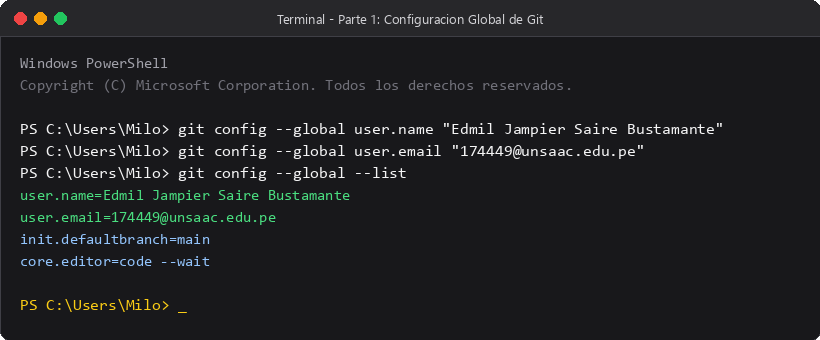
\includegraphics[width=0.92\textwidth]{capturas/captura1_config.png}
    \caption{Configuración de credenciales de usuario en Git.}
\end{figure}

\subsection{Parte 2: Creación del Proyecto e Inicialización}
Creé la carpeta para el proyecto de la startup (\texttt{pedidos-comida-cusco}), ingresé a ella e inicialicé el repositorio local con el comando \texttt{git init}. Configuré la rama principal como \texttt{main}.

\begin{terminalbox}{Comandos ejecutados}
mkdir pedidos-comida-cusco
cd pedidos-comida-cusco
git init
git branch -M main
\end{terminalbox}

\begin{figure}[H]
    \centering
    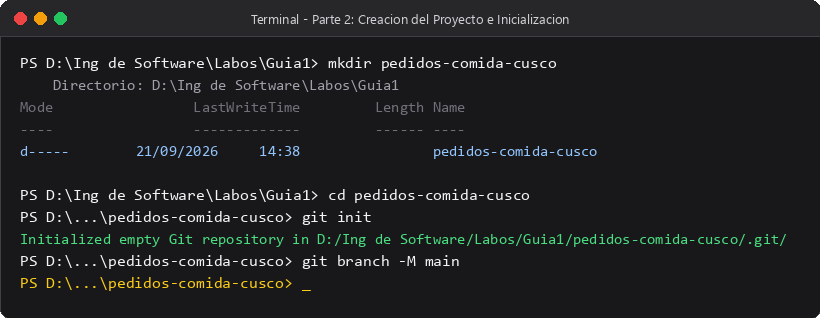
\includegraphics[width=0.92\textwidth]{capturas/captura2_init.png}
    \caption{Inicialización del repositorio Git local.}
\end{figure}

\subsection{Parte 3: Versionamiento Local y Primer Commit}
Creé el archivo \texttt{README.md} describiendo el proyecto. Verifiqué el estado con \texttt{git status}, pasé el archivo al área de preparación con \texttt{git add README.md} y realicé el commit inicial con un mensaje descriptivo.

\begin{terminalbox}{Comandos ejecutados}
git status
git add README.md
git commit -m "Primer commit: Estructura inicial del sistema de pedidos"
git log --oneline
\end{terminalbox}

\begin{figure}[H]
    \centering
    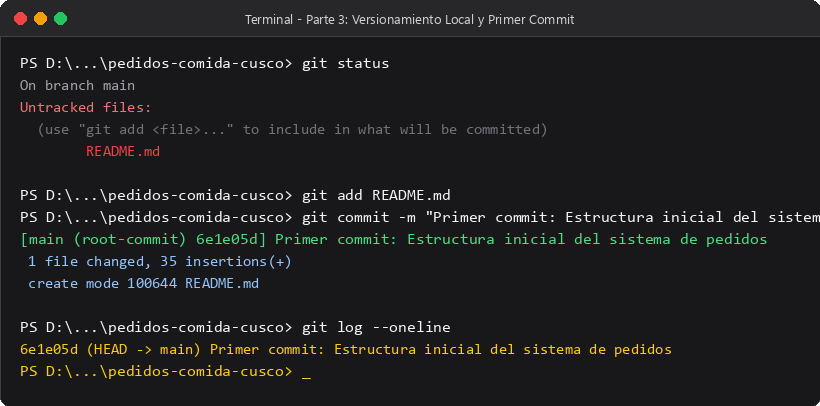
\includegraphics[width=0.92\textwidth]{capturas/captura3_commit.png}
    \caption{Inclusión del archivo al Staging Area y confirmación del commit.}
\end{figure}

\subsection{Parte 4: Repositorio Remoto en GitHub}
Creé el repositorio público \texttt{pedidos-comida-cusco} en mi cuenta de GitHub (\texttt{milith0kun}), vinculé el origen remoto a mi repositorio local y subí los cambios con \texttt{git push}.

\begin{terminalbox}{Comandos ejecutados}
git remote add origin https://github.com/milith0kun/pedidos-comida-cusco.git
git remote -v
git push -u origin main
\end{terminalbox}

\begin{figure}[H]
    \centering
    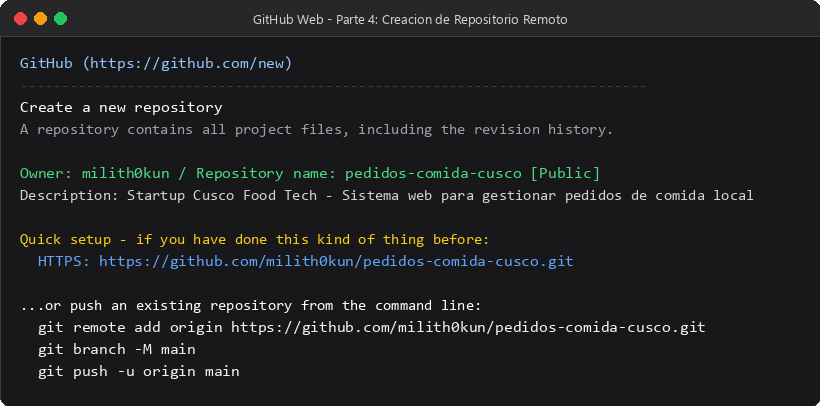
\includegraphics[width=0.92\textwidth]{capturas/captura4_crear_repo_github.png}
    \caption{Creación del repositorio en la interfaz web de GitHub.}
\end{figure}

\begin{figure}[H]
    \centering
    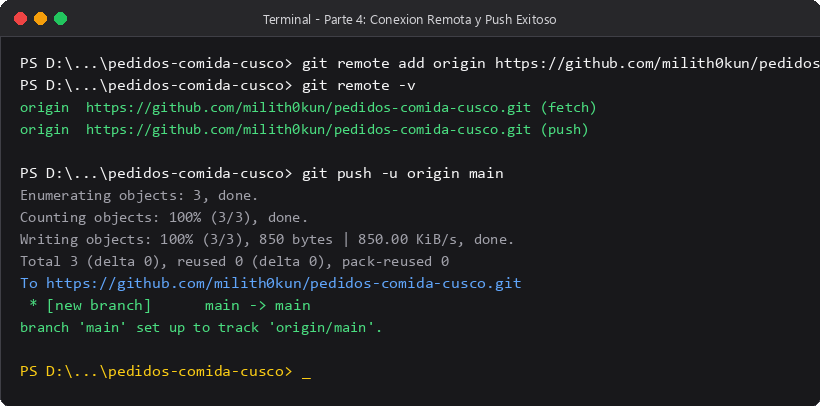
\includegraphics[width=0.92\textwidth]{capturas/captura5_push.png}
    \caption{Vinculación del origen remoto y envío exitoso con \texttt{git push}.}
\end{figure}

\begin{figure}[H]
    \centering
    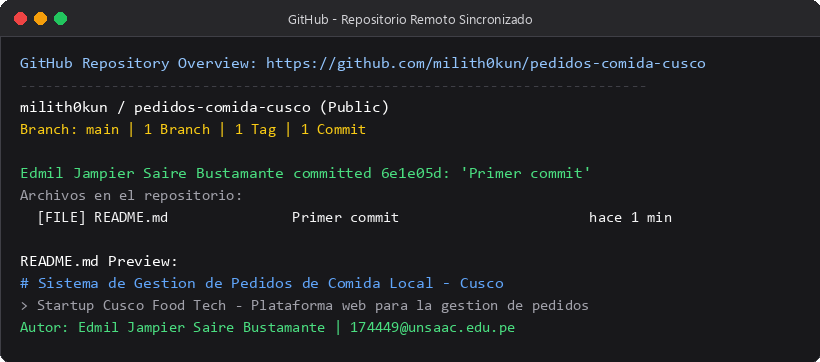
\includegraphics[width=0.92\textwidth]{capturas/captura6_evidencia_final.png}
    \caption{Vista del repositorio en GitHub con el archivo \texttt{README.md} subido.}
\end{figure}

% ==============================================================================
% 7. ENTREGABLES
% ==============================================================================
\section{Entregables}

\subsection{URL del Repositorio Remoto}
El proyecto se encuentra publicado en el siguiente enlace:
\begin{center}
    \url{https://github.com/milith0kun/pedidos-comida-cusco}
\end{center}

\subsection{Evidencia de Commits}
\begin{table}[H]
    \centering
    \begin{tabular}{@{}llllp{7cm}@{}}
        \toprule
        \textbf{Hash} & \textbf{Rama} & \textbf{Autor} & \textbf{Fecha} & \textbf{Mensaje} \\
        \midrule
        \texttt{6e1e05d} & \texttt{main} & Edmil Saire & 21/09/2026 & Primer commit: Estructura inicial del sistema de pedidos \\
        \texttt{32c5bc8} & \texttt{main} & Edmil Saire & 21/09/2026 & Docs: Mejorar documentacion del README \\
        \bottomrule
    \end{tabular}
    \caption{Registro de commits en el repositorio.}
\end{table}

\subsection{Documentación del Archivo README.md}
El archivo \texttt{README.md} incluye la descripción de la startup, la carta de platos cusqueños, la estructura y los comandos de clonación:
\begin{tcolorbox}[colback=codebg, colframe=unsaacblue!40, title=\textbf{Contenido del README.md}]
\small
\begin{verbatim}
# Sistema Web de Pedidos de Comida - Cusco
Proyecto inicial para la startup cusquena de pedidos de comida local.

## 1. Descripcion
Plataforma web para conectar picanterias del Cusco con clientes.

## 2. Platos considerados
* Chiri Uchu, Lechon Cusqueno, Kapchi de Setas, Cuy Chactado.

## 3. Estructura del Repositorio
pedidos-comida-cusco/
|-- README.md    # Documentacion tecnica inicial del proyecto

## 4. Clonacion
git clone https://github.com/milith0kun/pedidos-comida-cusco.git

Desarrollador: Edmil Jampier Saire Bustamante | 174449@unsaac.edu.pe | UNSAAC
\end{verbatim}
\end{tcolorbox}

% ==============================================================================
% 8. REFLEXIÓN
% ==============================================================================
\section{Reflexión}

\subsection{¿Por qué Git es crítico en proyectos colaborativos?}
Cuando varios compañeros trabajamos en un proyecto de software, enviarnos archivos por Drive, correo o WhatsApp genera confusión de inmediato. Git es indispensable porque:
\begin{itemize}
    \item \textbf{Permite trabajo paralelo:} Varios integrantes podemos programar distintas partes del sistema al mismo tiempo sin bloquearnos ni sobreescribir el trabajo de los demás.
    \item \textbf{Uso de ramas (\textit{branches}):} Cada miembro del equipo puede trabajar en una rama propia para probar una función y, cuando esté lista, integrarla de forma controlada a la rama principal.
    \item \textbf{Trazabilidad y autoría:} Cada cambio queda guardado con el nombre de quien lo hizo, la hora y el motivo, facilitando entender por qué se tomó cada decisión en el código.
\end{itemize}

\subsection{¿Qué problemas específicos evita el uso de Git?}
\begin{enumerate}
    \item \textbf{Sobreescritura accidental:} Evita que dos personas editen el mismo archivo y una borre sin querer lo que hizo la otra. Si hay líneas que chocan, Git avisa de un conflicto para resolverlo con calma.
    \item \textbf{Pérdida de avances funcionales:} Si al agregar algo nuevo el programa deja de funcionar, con Git podemos volver en segundos al commit anterior donde todo marchaba bien.
    \item \textbf{El desorden de versiones manuales:} Elimina la mala costumbre de guardar copias tipo \texttt{proyecto\_final}, \texttt{proyecto\_final\_v2}, \texttt{este\_si\_es\_el\_bueno.zip}. Todo el avance histórico se mantiene ordenado en una sola carpeta limpia.
    \item \textbf{Falta de control al subir cambios:} Facilita que antes de unir código a la rama principal se puedan hacer revisiones entre compañeros (Pull Requests) para detectar errores a tiempo.
\end{enumerate}

% ==============================================================================
% 9. CONCLUSIONES
% ==============================================================================
\section{Conclusiones}
\begin{itemize}
    \item Logré configurar mi entorno de desarrollo con Git en la terminal, enlazando mi nombre y correo institucional de la UNSAAC a cada commit.
    \item Comprendí en la práctica el flujo de trabajo en Git: modificar archivos en el directorio de trabajo, prepararlos con \texttt{git add} y confirmarlos con \texttt{git commit}.
    \item Conecté y sincronicé con éxito mi repositorio local con GitHub, cumpliendo con todos los entregables solicitados en la Guía 1.
\end{itemize}

\end{document}
